%! TeX program = lualatex
%! TEX options = -synctex=1 -interaction=nonstopmode -file-line-error --shell-escape "%DOC%"
\documentclass[a4paper,12pt]{article}
\usepackage{luatex85,shellesc}
\usepackage{luainputenc}
\usepackage{graphicx}
\usepackage{amsmath}
\usepackage{amssymb}
\usepackage[osf]{libertine}
\usepackage{enumerate}
\usepackage{enumitem}
\usepackage{tikz}
\usepackage[margin=1.6cm]{geometry}
\usepackage[hidelinks]{hyperref}
\usepackage{tcolorbox}
\usepackage{todonotes}
\usepackage{physics}
\usepackage{tikz}
\usepackage{float}
\usepackage{pgfplots}
\usepackage{wrapfig}
\usepackage{mathtools}

\usetikzlibrary{calc,backgrounds, decorations.pathmorphing}
\tikzset{snake it/.style={decorate, decoration=snake}}
\newcommand*\circled[1]{\tikz[baseline=(char.base)]{
            \node[shape=circle,draw,inner sep=2pt] (char) {#1};}}

\def\equationautorefname{Eq.}
\newcommand{\bs}[1]{\ensuremath{\boldsymbol{#1}}}
\DeclareMathOperator{\di}{d\!}
\setlength{\jot}{1em}

\renewcommand\thesubsection{\Alph{subsection}}

\newcommand{\mytitle}[1]{
	\begin{center}
		\Large \bf
		\textsc{#1}\\
		\vspace{-0.5em}
		\hspace*{0.2\linewidth} \hrulefill \hspace*{0.2\linewidth}
		\vspace{-0.5em}
	\end{center}
}

\newcommand{\mathunderline}[2]{\color{#1}\underline{{\color{black}#2}}\color{black}}

%%%%%%%%%%%%%%%%%%%%%%%%%%%%%%%%%%%%%%%%%%%%%%%

\begin{document}

% \mytitle{ASSIGMENT 1}

\section*{Problem 5}

\begin{wrapfigure}[12]{L}{0.5\linewidth}
    \centering
    \begin{tikzpicture}
        \pgfmathsetmacro{\h}{1.5}
        \pgfmathsetmacro{\ax}{0.5}
        \pgfmathsetmacro{\at}{0}
        \pgfmathsetmacro{\axx}{\ax}
        \pgfmathsetmacro{\att}{\h}
        \pgfmathsetmacro{\bx}{1.5}
        \pgfmathsetmacro{\bt}{0}
        \pgfmathsetmacro{\bxx}{\bx+0.5}
        \pgfmathsetmacro{\btt}{\h}
        \pgfmathsetmacro{\cx}{\ax}
        \pgfmathsetmacro{\ct}{\at}
        \pgfmathsetmacro{\cxx}{\ax + 0.5*\h}
        \pgfmathsetmacro{\ctt}{\at + 0.5*\h}
        \begin{axis}
            [
                axis lines  = center,
                xlabel={$x$},
                ylabel={$t$},
                xmin=-.1,
                xmax=2.5,
                ymin=-.1,
                ymax=2.5,
                xtick={-1},
                xticklabels={$g^{-1}$},
                ytick={-1}
                % ticks=none
            ]
            %
            \coordinate (A) at (axis cs:\ax, \at) {};
            \coordinate (AA) at (axis cs:\axx, \att) {};
            \coordinate (B) at (axis cs:\bx, \bt) {};
            \coordinate (BB) at (axis cs:\bxx, \btt) {};
            \coordinate (C) at (axis cs:\cx, \ct) {};
            \coordinate (CC) at (axis cs:\cxx, \ctt) {};
            %
            \draw[->] (A) -- (AA);
            \draw[->] (B) -- (BB);
            \draw[dotted, ->] (C) -- (CC);
            %
            \node[label={180:{$U^\mu$}},inner sep=2pt] at (AA) {};
            \node[label={0:{$V^\mu$}},inner sep=2pt] at (BB) {};
            \node[label={0:{$P^\mu$}},inner sep=2pt] at (CC) {};
        \end{axis}
    \end{tikzpicture}
    \caption{Setup of experiment}
    % \label{fig:zad1_1}
\end{wrapfigure}

We have given:
%
\begin{align}
    U^\mu & = \left(c,\bs{0}\right)                                       \\
    V^\mu & = \left(\gamma_v c,\gamma_v \bs{v}\right) \label{eq:zad1_vel} \\
    P^\mu & = \left(\frac{h\nu}{c},\bs{p}\right)
\end{align}

We use following relation in this problem:
%
\begin{equation}
    E = -P^\mu V_\mu
\end{equation}
%
This expression is Lorentz invariant and can be calculated in non-moving frame.
So we plug in \autoref{eq:zad1_vel} in this expression to obtain
%
\begin{multline}
    E = -P^\mu V_\mu = \frac{h\nu}{c}\gamma_v c - \gamma_v \bs{v}\bs{p} = 
    \gamma_v\left(h\nu - |\bs{v}||\bs{p}|\cos(\theta)\right) = 
    \left\{|\bs{p}| = \frac{h\nu}{c}\right\} =\\
    \gamma_vh\nu\left(1-\frac{|\bs{v}|}{c}\cos(\theta)\right)
\end{multline}
%
But it is still photon, but with different energy (for moving observer) So
%
\begin{equation}
    \gamma_vh\nu\left(1-\frac{|\bs{v}|}{c}\cos(\theta)\right) = h\nu'
\end{equation}
%
So ratio of those two frequencies is
%
\begin{equation}
    \frac{\nu'}{\nu} = \gamma_v\left(1-\frac{|\bs{v}|}{c}\cos(\theta)\right)
\end{equation}
%
If $\theta = 0$ and $\frac{v}{c} \ll 1 \Rightarrow \gamma_v \simeq 1$ then we
obtain:
%
\begin{equation}
    \boxed{\nu' = \nu \left(1-\frac{v}{c}\right)}
\end{equation}

\newpage

\mytitle{ASSIGMENT 2}

\section*{Problem 1a}

\begin{wrapfigure}[16]{L}{0.5\linewidth}
    \centering
    \begin{tikzpicture}
        \pgfmathsetmacro{\h}{5}
        \pgfmathsetmacro{\w}{5}
        \pgfmathsetmacro{\err}{0.2}
        \pgfmathsetmacro{\ax}{0}
        \pgfmathsetmacro{\ay}{\h}
        \pgfmathsetmacro{\bx}{0}
        \pgfmathsetmacro{\by}{0}
        \pgfmathsetmacro{\cx}{\w}
        \pgfmathsetmacro{\cy}{0}
        \pgfmathsetmacro{\dx}{\w}
        \pgfmathsetmacro{\dy}{\h}

        \coordinate (A) at (\ax, \ay) {};
        \coordinate (B) at (\bx, \by) {};
        \coordinate (C) at (\cx, \cy) {};
        \coordinate (D) at (\dx, \dy) {};
        %
        \draw[->] ($(A)+(0,-\err)$) -- node [text width=1cm, midway,align=left]{h} ($(B)+(0,\err)$);
        \draw[->, dotted] ($(B)+(\err,0)$) -- ($(C)+(-\err,0)$);
        \draw[->, snake it] ($(C)+(0,\err)$) -- ($(D)+(0,-\err)$);
        \draw[->, dotted] ($(D)+(-\err,0)$) -- ($(A)+(\err,0)$);
        %
        \node[label={90:{\circled{1}}}, circle, fill, inner sep=2pt] at (A) {};
        \node[label={270:{\circled{2}}}, circle, fill, inner sep=2pt] at (B) {};
        \node[label={270:{\circled{3}}}, draw, dashed, circle, inner sep=2pt] at (C) {};
        \node[label={90:{\circled{4}}}, draw, dashed, circle, inner sep=2pt] at (D) {};
    \end{tikzpicture}
    \caption{Mass falling in graitational field (1\rightarrow 2), converting to
    photon (2\rightarrow 3), photon traveling up (3\rightarrow 4) and converting
    back to mass (4\rightarrow 1)}
    % \label{fig:zad1_1}
\end{wrapfigure}

Let's take a look at energy changes in above diagram:
\begin{enumerate}[label=\protect\circled{\arabic*}]
    \item $E_1 = mc^2$
    \item $E_2 = mc^2 + mgh$
    \item $E_3 = h\nu = mc^2 + mgh$
    \item $E_4 = h\nu = mc^2 + mgh$
\end{enumerate}
but $E_4 = E_1$ because of energy conservation. It means that photon has to have
different frequency at the height $h$ than it has at the ground. So $E_4 = h\nu'
= mc^2$. From it follows
%
\begin{equation}
    \frac{\nu}{\nu'} = \frac{mc^2+mgh}{mc^2} = 1 + \frac{gh}{c^2}
\end{equation}
%
and it is easy to calculate redshift 
%
\begin{equation}
    \boxed{z = \frac{\nu - \nu'}{\nu'} = \frac{gh}{c^2}}
    \label{eq:prob2a_res}
\end{equation}

\section*{Problem 1b}

\begin{wrapfigure}[16]{R}{0.5\linewidth}
    \centering
    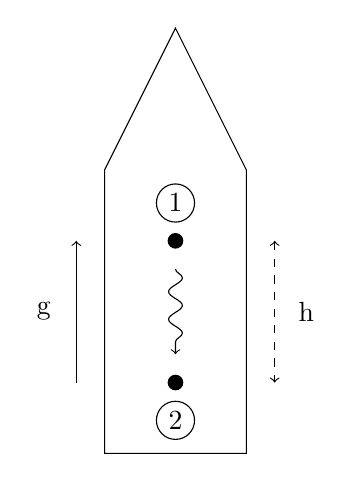
\begin{tikzpicture}[scale=1.8]
        \draw (0,0) -- (0,2) -- (0.5,3) -- (1,2) -- (1, 0) -- cycle;
        \draw[->, snake it] (0.5, 1.3) -- (0.5, 0.7);
        \draw[<->, dashed] (1.2, 1.5) -- node [text width=1cm, midway,align=right]{h}(1.2, 0.5);
        \draw[<-] (-.2, 1.5) -- node [text width=1cm, midway,align=left]{g}(-.2, 0.5);
        %
        \node[label={90:{\circled{1}}}, circle, fill, inner sep=2pt] at (0.5, 1.5) {};
        \node[label={270:{\circled{2}}}, circle, fill, inner sep=2pt] at (0.5, 0.5) {};
    \end{tikzpicture}
    \caption{Two observers in a rocket sending photon}
    % \label{fig:zad1_1}
\end{wrapfigure}

Let's calculate time which light needs to reach observer \circled{2}
%
\begin{equation}
    t = \frac{s}{c} = \frac{h - \frac{gt^2}{2}}{c}
\end{equation}
%
From this expression we get quadratic equation 
%
\begin{equation}
    \frac{g}{2}t^2 + ct - h = 0
\end{equation}
%
for which solution is given by
%
\begin{equation}
    t = \frac{-c + \sqrt{c^2+2gh}}{g}
\end{equation}
%
Velocity of observer \circled{2} after this time is equal 
%
\begin{equation}
    v(t) = \frac{-c + \sqrt{c^2+2gh}}{g} \cdot g = -c + \sqrt{c^2+2gh}
\end{equation}
%
Then redshift formula is given in following way
%
\begin{equation}
    \frac{\nu'}{\nu} = 1 - \frac{v}{c} = 1 - \frac{-c + \sqrt{c^2+2gh}}{c} = 
    2 - \sqrt{1-\frac{2gh}{c^2}} 
\end{equation}
%
We can use Taylor expansion $\sqrt{1-x} = 1-\frac{x}{2}$ we get
%
\begin{equation}
    \boxed{\frac{\nu'}{\nu} = 2 - 1 + \frac{gh}{c^2} = 1 + \frac{gh}{c^2} }
\end{equation}
%
It is exactly the same result as \autoref{eq:prob2a_res}.

% \problem

Observer $\mathcal{O}$ is traveling with acceleration $g$ in direction $x_1$. To
calculate his worldline we will use following three conditions
%
\begin{align}
	U^\mu U_\mu & = -1 & U^\mu A_\mu & = 0 & A^\mu A_\mu & = g^2
\end{align}
%
where $U^\mu$ is four-velocity and $A^\mu$ is four-acceleration. First of them
can be obtained by straightforward calculation, second by applying derivative
to first equation i.e.
%
\begin{equation}
	\frac{\dd}{\dd \tau} \left(U^\mu U_\mu\right) = 0 \quad \Rightarrow \quad \left(A^\mu U_\mu\right) = 0
\end{equation}
%
Third is Lorentz invariant and it can be calculated in the moment of launch
namely when $A^\mu=(0,g,0,0)$.

Knowing those three we can write them in explicite form
\begin{align}
	-U_0^2 + \boldsymbol{U}^2    & = -1      &
	\boldsymbol{U}\boldsymbol{A} & = U_0 A_0 &
	-A_0^2 + \boldsymbol{A}^2    & = g^2
\end{align}
%
where bolded letters mean three-vectors.

We square middle equation and plug in left and right equation to obtained
%
\begin{equation}
	(U_0^2 - 1)\boldsymbol{A}^2  = U_0^2  (\boldsymbol{A}^2 -g^2)
\end{equation}
%
Eventually we obtain:
%
\begin{equation}
	\boldsymbol{A}^2 = g^2 U_0^2
\end{equation}
%
and plugin this expression to other equation we also obtain:\footnote{plug it
	into right equation and then use left equation}
%
\begin{equation}
	A_0^2 = g^2 \boldsymbol{U}^2
\end{equation}
%
We can simplify those equation using the fact that this motion is one
dimensional namely $x_2=x_3=0$ and then
%
\begin{align}
	A_1 & = g U_0 & A_0 & = g U_1
\end{align}
%
But $U^\mu = \dot{X^\mu}$ and $A^\mu = \ddot{X^\mu}$ \footnote{dot means
	derivation with respect to proper time}. Substituting
%
\begin{align}
	\ddot{X_1} & = g \dot{X_0} & \ddot{X_0} & = g \dot{X_1}
\end{align}
%
Taking a derivative of left equation and substituting right equation into it we
get
%
\begin{equation}
	\dddot{X_1} = g^2 \dot{X_1}
	\quad \stackrel{\text{after integration}}{\Rightarrow} \quad
	\ddot{X_1} = g^2 X_1
\end{equation}
%
Solution is
%
\begin{equation}
	X_1 = A \sinh(g\tau) + B \cosh(g\tau)
\end{equation}
%
Let's choose initial conditions such as $X_1(0) = g^{-1}$ and $\dot{X_1}=0$. Then
%
\begin{equation}
	X_1 = g^{-1} \cosh(g\tau)
\end{equation}
%
And finally we have
%
\begin{align}
	X_0 & = g^{-1} \sinh(g\tau) & X_1 & = g^{-1} \cosh(g\tau) & X_2 & = 0 & X_3 & = 0
	\label{eq:hiper}
\end{align}
%
\begin{figure}[H]
	\centering
	\begin{tikzpicture}[domain=0:20]
		\pgfmathsetmacro{\g}{1.5}
		\pgfmathsetmacro{\gg}{1/\g}
		\begin{axis}
			[
				axis lines  = center,
				xlabel={$x$},
				ylabel={$t$},
				xmin=0,
				xmax=2.5,
				ymin=0,
				ymax=2.5,
				xtick={\gg},
				xticklabels={$g^{-1}$},
				ytick={-1}
				% ticks=none
			]

			\pgfmathsetmacro{\a}{1.1}
			\pgfmathsetmacro{\ta}{\gg*cosh(\g*\a)}
			\pgfmathsetmacro{\xa}{\gg*sinh(\g*\a)}

			\pgfmathsetmacro{\b}{.1}
			\pgfmathsetmacro{\tb}{\gg*cosh(\g*\b)}
			\pgfmathsetmacro{\xb}{\gg*sinh(\g*\b)}

			\pgfmathsetmacro{\tav}{\gg*cosh(\g*(\a+\b)/2)}
			\pgfmathsetmacro{\xav}{\gg*sinh(\g*(\a+\b)/2)}

			\pgfmathsetmacro{\tp}{\tav*e^(\g*(\a-\b)/2)}
			\pgfmathsetmacro{\xp}{\xav*e^(\g*(\a-\b)/2)}
			%wektory bazowe
			\pgfmathsetmacro{\ezerot}{\ta+cosh(\g*\a)}
			\pgfmathsetmacro{\ezerox}{\xa+sinh(\g*\a)}
			\pgfmathsetmacro{\eonet}{\ta+sinh(\g*\a)}
			\pgfmathsetmacro{\eonex}{\xa+cosh(\g*\a)}

			\coordinate (A) at (axis cs:\ta, \xa) {};
			\coordinate (B) at (axis cs:\tb, \xb) {};
			\coordinate (C) at (axis cs:\tp, \xp) {};
			\coordinate (D) at (axis cs:\tav, \xav) {};
			\coordinate (E) at (axis cs:0,0) {};
			%baza
			\coordinate (ezero) at (axis cs:\ezerot,\ezerox) {};
			\coordinate (eone) at (axis cs:\eonet,\eonex) {};

			\addplot[domain = 0:2.8*\gg, parametric, samples = 1000,color=blue]
			gnuplot {\gg*cosh(\g*t),\gg*sinh(\g*t)};

			% \node[label={180:{$\tau_2$}},circle,fill,inner sep=2pt] at (A) {};
			% \node[label={180:{$\tau_1$}},circle,fill,inner sep=2pt] at (B) {};
			% \node[label={360:{\color{red}$P$}},circle,fill,inner sep=2pt,color=red] at (C) {};
			% \node[label={160:{\color{red}$\frac{\tau_1+\tau_2}{2}$}},circle,fill,inner sep=2pt,color=red] at (D) {};

		\end{axis}
		\begin{scope}[on background layer]
			% \draw[dashed] (A) -- (C);
			% \draw[dashed] (B) -- (C);
			% \draw[dotted,color=red] (C) -- (E);
			%baza
			% \draw[->] (A) -- (ezero);
			% \draw[->] (A) -- (eone);
		\end{scope}
	\end{tikzpicture}
	\caption{Trajectory of $\mathcal{O}$}
	\label{fig:zad1}
\end{figure}

% \bigskip

\problem
%
As a first basis vector we can choose four-velocity namely
%
\begin{equation}
	\boldsymbol{e}_0 = \left(\dot{X_0}, \dot{X_1}, \dot{X_2}, \dot{X_3}\right) =
	\left(\cosh(g\tau), \sinh(g\tau), 0, 0\right)
\end{equation}
%
As a basis vectors in directions $x_2$ and $x_3$ we simply choose
%
\begin{align}
	\boldsymbol{e}_2 = \left(0, 0, 1, 0\right) \\
	\boldsymbol{e}_3 = \left(0, 0, 0, 1\right)
\end{align}
%
And finally we choose vector $\boldsymbol{e}_1$ in a form $\boldsymbol{e}_1 =
	\left(e_1^0, e_1^1, 0, 0\right)$ where $e_1^0$ and $e_1^1$ are chosen in order
to satisfy $\boldsymbol{e}_0 \boldsymbol{e}_1 = 0$ and $(\boldsymbol{e}_0)^2=1$ i.e.
%
\begin{align}
	-e_1^0 \cosh(g\tau) + e_1^1 \sinh(g\tau) & = 0 \\
	-(e_1^0)^2 + (e_1^1)^2 = 1
\end{align}
%
We square first equation and substitute second equation
%
\begin{equation}
	(e_1^0)^2 \cosh^2(g\tau) = (1+(e_1^0)^2) \sinh^2(g\tau)
\end{equation}
%
From this we obtain
%
\begin{align}
	(e_1^0)^2 & = \sinh^2(g\tau) & (e_1^1)^2 & = \cosh^2(g\tau)
\end{align}
%
We can choose positive solution and eventually we get
%
\begin{equation}
	\boldsymbol{e}_1 = \left(\sinh(g\tau), \cosh(g\tau), 0, 0\right)
\end{equation}
%
All vectors
%
\begin{align}
	\boldsymbol{e}_0(\tau) & = \left(\cosh(g\tau), \sinh(g\tau), 0, 0\right) \\
	\boldsymbol{e}_1(\tau) & = \left(\sinh(g\tau), \cosh(g\tau), 0, 0\right) \\
	\boldsymbol{e}_2(\tau) & = \left(0, 0, 1, 0\right)                       \\
	\boldsymbol{e}_3(\tau) & = \left(0, 0, 0, 1\right)
\end{align}
%
Last thing to do is to check whether those are vectors which were obtain without
any rotation. For this I will find a Lorentz boost which transforms initial
basis into this one. Namely consider a boost of time-basis vector

\begin{equation}
	\begin{pmatrix}
		\gamma       & \beta\gamma & 0 & 0 \\
		-\beta\gamma & \gamma      & 0 & 0 \\
		0            & 0           & 1 & 0 \\
		0            & 0           & 0 & 1
	\end{pmatrix}
	\begin{pmatrix}
		1 \\
		0 \\
		0 \\
		0
	\end{pmatrix}
	=
	\begin{pmatrix}
		\gamma       \\
		-\beta\gamma \\
		0            \\
		0
	\end{pmatrix}
\end{equation}
%
So $\gamma$ and $\beta$ have to satisfy:
%
\begin{equation}
	\gamma = \frac{1}{\sqrt{1-v^2}} = \cosh(g\tau) \quad \Rightarrow \quad v = \tanh(g\tau)
\end{equation}
%
Knowing that it is easy to calculate
%
\begin{equation}
	\beta\gamma = \frac{v}{\sqrt{1-v^2}} = \sinh(g\tau)
\end{equation}
%
So indeed we obtain vector $\boldsymbol{e}_0(\tau)$ only via boost (at
$v=\tanh(g\tau)$). The same can be done with vector $\boldsymbol{e}_1(\tau)$

\problem

We define new coordinate system $(\xi_0\equiv\tau, \xi_1, \xi_2, \xi_3)$ where
basis vectors are those defined in problem before. We can write
%
\begin{equation}
	\boldsymbol{x} = \xi^1\boldsymbol{e}_1(\tau) + \xi^2\boldsymbol{e}_2(\tau) +
	\xi^3\boldsymbol{e}_3(\tau) + \boldsymbol{x}_\mathcal{O}(\tau)
\end{equation}
%
where $\boldsymbol{x}_\mathcal{O}(\tau)$ is trajectory of moving frame.

After plugging in all basis vectors explicitly we get
%
\begin{multline}
	\boldsymbol{x} =
	\begin{pmatrix}
		t   \\
		x_1 \\
		x_2 \\
		x_3
	\end{pmatrix}
	=
	\begin{pmatrix}
		\xi^1 \sinh(g\tau) \\
		\xi^1 \cosh(g\tau) \\
		0                  \\
		0
	\end{pmatrix}+
	\begin{pmatrix}
		0     \\
		0     \\
		\xi^2 \\
		0
	\end{pmatrix}+
	\begin{pmatrix}
		0 \\
		0 \\
		0 \\
		\xi^3
	\end{pmatrix}+
	\begin{pmatrix}
		g^{-1}\sinh(g\tau) \\
		g^{-1}\cosh(g\tau) \\
		0                  \\
		0
	\end{pmatrix}= \\
	\begin{pmatrix}
		g^{-1}\sinh(g\tau) + \xi^1 \sinh(g\tau) \\
		g^{-1}\cosh(g\tau) + \xi^1 \cosh(g\tau) \\
		\xi^2                                   \\
		\xi^3
	\end{pmatrix}
	=
	\begin{pmatrix}
		(g^{-1} + \xi^1) \sinh(g\xi^0) \\
		(g^{-1} + \xi^1) \cosh(g\xi^0) \\
		\xi^2                          \\
		\xi^3
	\end{pmatrix}
	\label{eq:motion}
\end{multline}
%
Line element $\dd s^2 = \eta_{\mu\nu} \dd x^\mu \dd x^\nu$ is then equal (we use
chain rule i.e. $\dd x^\mu = \frac{\partial x^\mu}{\partial \xi^\nu}\dd
	\xi^\nu$)
%
\begin{equation}
	\dd s^2 = - \dd t^2 + \dd x_1^2 + \dd x_2^2 + \dd x_3^2
\end{equation}
\begin{align}
	\dd t   & = \frac{\partial t}{\partial \xi^\nu}\dd \xi^\nu =
	(1 + g\xi_1)\cosh(g\xi_0) \dd \xi_0 + \sinh(g\xi_0) \dd \xi_1             \\
	\dd x_1 & = (1 + g\xi_1)\sinh(g\xi_0) \dd \xi_0 + \cosh(g\xi_0) \dd \xi_1 \\
	\dd x_2 & = \dd \xi_2                                                     \\
	\dd x_3 & = \dd \xi_3
\end{align}
After squaring and adding them up we get
%
\begin{align}
	\dd s^2 =  - & (1 + g\xi_1)^2\cosh^2(g\xi_0) \dd \xi_0^2 - \sinh^2(g\xi_0) \dd \xi_1^2 +           \\
	             & (1 + g\xi_1)^2\sinh^2(g\xi_0) \dd \xi_0^2 + \cosh^2(g\xi_0) \dd \xi_1^2 + \nonumber \\
	             & \dd \xi_2^2 +                                                             \nonumber \\
	             & \dd \xi_3^2 \nonumber
\end{align}
After simplification
\begin{equation}
	\boxed{\dd s^2 = -(1+g\xi_1)^2\dd\xi_0^2 + \dd\xi_1^2 + \dd\xi_2^2 + \dd\xi_3^2}
	\label{eq:action}
\end{equation}

\problem

For $\xi^1 \equiv \text{const}$ we can easily derive equation of motion from
\autoref{eq:motion} namely
%
\begin{equation}
	x_1^2 - t^2 = (g^{-1}+\xi^1)^2
\end{equation}
%
which leads to
%
\begin{equation}
	x_1(t) = \sqrt{(g^{-1}+\xi^1)^2 + t^2}
	\label{eq:sqrt}
\end{equation}
%
We take derivative twice
%
\begin{align}
	\dot{x_1}(t)  & = \frac{2t}{2\sqrt{(g^{-1}+\xi^1)^2 + t^2}} \\
	\ddot{x_1}(t) & =
	\frac{\sqrt{(g^{-1}+\xi^1)^2 + t^2} -
		t \frac{2t}{2\sqrt{(g^{-1}+\xi^1)^2 + t^2}}}{(g^{-1}+\xi^1)^2 + t^2} =
	\frac{1}{\sqrt{(g^{-1}+\xi^1)^2 + t^2}} -
	\frac{2t^2}{((g^{-1}+\xi^1)^2 + t^2)^{\frac{3}{2}}}
\end{align}
%
So when $t=0$
%
\begin{equation}
	\boxed{\ddot{x_1}(t)\Big|_{t=0} = \frac{1}{g^{-1}+\xi^1} = \frac{g}{1+g\xi^1}}
\end{equation}


\begin{figure}[H]
	\centering
	\foreach \angle in {0,0.1,0.2}
		{
			\resizebox{0.3\linewidth}{0.3\linewidth}{
				\begin{tikzpicture}[domain=0:5]
					\pgfmathsetmacro{\g}{1.5}
					\pgfmathsetmacro{\gg}{1/\g}
					\pgfmathsetmacro{\xii}{0.5}
					\pgfmathsetmacro{\ggxi}{\gg+\xii}
					\begin{axis}
						[
							axis lines  = center,
							xlabel={$x$},
							ylabel={$t$},
							xmin=-0.1,
							xmax=2.5,
							ymin=-0.1,
							ymax=2.5,
							xtick={\gg,\ggxi},
							xticklabels={$g^{-1}$,$g^{-1}+\xi^1$},
							ytick={-1}
							% ticks=none,
						]

						\pgfmathsetmacro{\g}{1.5}
						\pgfmathsetmacro{\gg}{1/\g}

						\pgfmathsetmacro{\a}{\angle}
						\pgfmathsetmacro{\ta}{\gg*cosh(\g*\a)}
						\pgfmathsetmacro{\xa}{\gg*sinh(\g*\a)}

						\pgfmathsetmacro{\aa}{\angle}
						\pgfmathsetmacro{\taa}{\ggxi*cosh(\g*\aa)}
						\pgfmathsetmacro{\xaa}{\ggxi*sinh(\g*\aa)}

						\pgfmathsetmacro{\b}{.1}
						\pgfmathsetmacro{\tb}{\gg*cosh(\g*\b)}
						\pgfmathsetmacro{\xb}{\gg*sinh(\g*\b)}

						\pgfmathsetmacro{\tav}{\gg*cosh(\g*(\a+\b)/2)}
						\pgfmathsetmacro{\xav}{\gg*sinh(\g*(\a+\b)/2)}

						\pgfmathsetmacro{\tp}{\tav*e^(\g*(\a-\b)/2)}
						\pgfmathsetmacro{\xp}{\xav*e^(\g*(\a-\b)/2)}
						%wektory bazowe
						\pgfmathsetmacro{\ezerot}{\ta+cosh(\g*\a)}
						\pgfmathsetmacro{\ezerox}{\xa+sinh(\g*\a)}
						\pgfmathsetmacro{\eonet}{\ta+sinh(\g*\a)}
						\pgfmathsetmacro{\eonex}{\xa+cosh(\g*\a)}

						\coordinate (A) at (axis cs:\ta, \xa) {};
						\coordinate (AA) at (axis cs:\taa, \xaa) {};
						\coordinate (B) at (axis cs:\tb, \xb) {};
						\coordinate (C) at (axis cs:\tp, \xp) {};
						\coordinate (D) at (axis cs:\tav, \xav) {};
						\coordinate (E) at (axis cs:0,0) {};
						%baza
						\coordinate (ezero) at (axis cs:\ezerot,\ezerox) {};
						\coordinate (eone) at (axis cs:\eonet,\eonex) {};

						% \addplot[domain = 0:1.7, samples=1000, parametric, color=blue]
						% gnuplot {sqrt((\ggxi)^2+t^2),t};	
						\addplot[domain = 0:0.9, parametric, samples = 1000,color=blue]
						gnuplot {\ggxi*cosh(\g*t),\ggxi*sinh(\g*t)};
						\addplot[domain = 0:1.3, parametric, samples = 1000,color=red]
						gnuplot {\gg*cosh(\g*t),\gg*sinh(\g*t)};

						\node[label={180:{${}$}},circle,fill,inner sep=2pt] at (A) {};
						\node[label={180:{${}$}},circle,fill,inner sep=2pt] at (AA) {};
						% \node[label={180:{$\tau_1$}},circle,fill,inner sep=2pt] at (B) {};
						% \node[label={360:{\color{red}$P$}},circle,fill,inner sep=2pt,color=red] at (C) {};
						% \node[label={160:{\color{red}$\frac{\tau_1+\tau_2}{2}$}},circle,fill,inner sep=2pt,color=red] at (D) {};

					\end{axis}
					\begin{scope}[on background layer]
						% \draw[dashed] (A) -- (C);
						% \draw[dashed] (B) -- (C);
						% \draw[dotted,color=red] (C) -- (E);
						%baza
						\draw[->] (A) -- (ezero);
						\draw[->] (A) -- (eone);
						% \draw[dotted] (A)+(3,3) -- (A);
					\end{scope}
				\end{tikzpicture}}
		}
	\caption{\textcolor{red}{Red} line is worldline of \autoref{eq:hiper}
		and \textcolor{blue}{blue} is worldline of \autoref{eq:sqrt}}
	\label{fig:zad4}
\end{figure}

\problem

We start with equation \autoref{eq:action}. We can simplify it and neglect other
spatial dimensions than $\xi^1$ namely
%
\begin{equation}
	\dd s^2 = -(1+g\xi^1)^2 (\dd\xi^0)^2 + (\dd\xi^1)^2
\end{equation}
%
We can change the form to
%
\begin{equation}
	\dd \tau = \dd s = \dd\xi^0 \sqrt{-(1+g\xi^1)^2 + \left(\frac{\dd\xi^1}{\dd\xi^0}\right)^2}
\end{equation}
%
We can now plug in $\xi^1 = \xi^1_\text{em}$ and since emiter does not move in
this frame we can set $\frac{\dd\xi^1}{\dd\xi^0} = 0$:
%
\begin{equation}
	\dd \tau_\text{em} = \dd\xi^0_\text{em} (1+g\xi^1_\text{em})
\end{equation}
%
We can integrate both sides and obtain equation for finite differences
%
\begin{equation}
	\Delta \tau_\text{em} = \Delta \xi^0_\text{em} (1+g\xi^1_\text{em})
\end{equation}
%
We can do similar thing with $\xi^1_\text{rec}$:
%
\begin{equation}
	\Delta \tau_\text{rec} = \Delta \xi^0_\text{rec} (1+g\xi^1_\text{rec})
\end{equation}
%
But left sides of above equations are equal (since line element is invariant
under changing of coordinates) and we can compare them:
%
\begin{equation}
	\frac{\Delta \xi^0_\text{rec}}{\Delta \xi^0_\text{em}} =
	\frac{1+g\xi^1_\text{em}}{1+g\xi^1_\text{rec}} =
	1 + \frac{g\xi^1_\text{em} - g\xi^1_\text{rec}}{1+g\xi^1_\text{rec}} =
	1 - \frac{gh}{1+gh+g\xi^1_\text{em}}
\end{equation}
%
where I put $h = \xi^1_\text{rec} - \xi^1_\text{em}$. After rearranging terms and
substituting $\Delta \xi_\text{rec}^1 = \frac{1}{\nu'}$ and $\Delta
	\xi_\text{em}^1 = \frac{1}{\nu}$
%
\begin{equation}
	\frac{\Delta \xi^0_\text{em} - \Delta \xi^0_\text{rec}}{\Delta \xi^0_\text{em}} =
	\frac{gh}{1+gh+g\xi^1_\text{em}}
\end{equation}
%
\begin{equation}
	\frac{\frac{1}{\nu} - \frac{1}{\nu'}}{\frac{1}{\nu}} =
	\frac{gh}{1+gh+g\xi^1_\text{em}}
	\quad \Rightarrow \quad
	\boxed{z = \frac{\nu' - \nu}{\nu'} = \frac{gh}{1+gh+g\xi^1_\text{em}}}
\end{equation}
%
We can now assume that $g$ is small and using Taylor expansion $\frac{1}{1+x}
	\simeq 1-x$
%
\begin{gather}
	z = gh(1-gh-g\xi^1_\text{em}) = gh - (gh)^2 - g^2h\xi^1_\text{em} \simeq gh \nonumber \\
	z = gh
\end{gather}
%
so the same result as photon in gravitational field.

% \mytitle{assigment 3}

\section*{Problem 1}

\begin{equation}
    \mathcal{L}(x^\mu,\dot{x}^\mu) =
    \frac{1}{2}g_{\mu\nu}[x^\mu(\lambda)]\dot{x}^\mu\dot{x}^\nu, \quad
    \dot{x}^{\mu} \equiv \frac{\di x^\mu}{\dd\lambda}
\end{equation}

\begin{multline}
    \delta\int\limits_{\lambda1}^{\lambda2}\mathcal{L}(x^\mu,\dot{x}^\mu)\dd\lambda =
    \int\limits_{\lambda1}^{\lambda2}
    \left(\frac{\partial\mathcal{L}(x^\mu,\dot{x}^\mu)}{\partial x^\sigma}\delta x^\sigma +
    \frac{\partial\mathcal{L}(x^\mu,\dot{x}^\mu)}{\partial \dot{x}^\sigma}\delta \dot{x}^\sigma\right)\dd\lambda = \\
    \int\limits_{\lambda1}^{\lambda2}
    \left(\frac{1}{2}\dot{x}^\mu\dot{x}^\nu \partial_\sigma g_{\mu\nu} \delta x^\sigma +
    \frac{1}{2}g_{\mu\nu}(\delta_{\mu\sigma} \dot{x}^\nu + \delta_{\nu\sigma} \dot{x}^\mu)\delta \dot{x}^\sigma\right)\dd\lambda
\end{multline}
%
Let's take a look at second part of the integral:
%
\begin{multline}
    \frac{1}{2}\int\limits_{\lambda1}^{\lambda2}
    \left\{g_{\mu\nu}(\delta_{\mu\sigma}
    \dot{x}^\nu + \delta_{\nu\sigma} \dot{x}^\mu)\delta \dot{x}^\sigma\right\}\dd\lambda =
    %
    \frac{1}{2}\int\limits_{\lambda1}^{\lambda2}
    \left\{g_{\sigma\nu}\dot{x}^\nu + g_{\mu\sigma}\dot{x}^\mu \right\}
    \delta\dot{x}^\sigma\dd\lambda = \\
    %
    \frac{1}{2}\int\limits_{\lambda1}^{\lambda2}
    \frac{\partial}{\partial\lambda}\left(\left\{
    g_{\sigma\nu}\dot{x}^\nu + g_{\mu\sigma}\dot{x}^\mu
    \right\}\delta x^\sigma\right)\dd\lambda -
    \frac{1}{2}\int\limits_{\lambda1}^{\lambda2}
    \frac{\partial}{\partial\lambda}\left\{
    g_{\sigma\nu}\dot{x}^\nu + g_{\mu\sigma}\dot{x}^\mu
    \right\}\delta x^\sigma\dd\lambda= \\
    %
    \frac{1}{2}\underbrace{\left\{g_{\sigma\nu}\dot{x}^\nu + g_{\mu\sigma}\dot{x}^\mu\right\} \delta x^\sigma \Bigg|_{\lambda1}^{\lambda2}}_{=0} -
    \frac{1}{2}\int\limits_{\lambda1}^{\lambda2}
    \left\{
    \partial_{\mu}g_{\sigma\nu}\dot{x}^\mu\dot{x}^\nu + g_{\sigma\nu}\ddot{x}^\nu +
    \partial_{\nu}g_{\sigma\mu}\dot{x}^\nu\dot{x}^\mu + g_{\sigma\mu}\ddot{x}^\mu
    \right\}\delta x^\sigma\dd\lambda \\
    %
\end{multline}
\begin{equation}
    \delta\int\limits_{\lambda1}^{\lambda2}\mathcal{L}(x^\mu,\dot{x}^\mu)\dd\lambda =
    \frac{1}{2}\int\limits_{\lambda1}^{\lambda2}
    \left(\partial_\sigma g_{\mu\nu}\dot{x}^\mu\dot{x}^\nu -
    \partial_{\mu}g_{\sigma\nu}\dot{x}^\mu\dot{x}^\nu - g_{\sigma\nu}\ddot{x}^\nu -
    \partial_{\nu}g_{\sigma\mu}\dot{x}^\nu\dot{x}^\mu - g_{\sigma\mu}\ddot{x}^\mu\right)\delta x^\sigma \dd\lambda
\end{equation}
%
We want
%
\begin{equation}
    \delta\int\limits_{\lambda1}^{\lambda2}\mathcal{L}(x^\mu,\dot{x}^\mu)\dd\lambda = 0
\end{equation}
%
but since $\delta x^\sigma$ can be arbitrary the rest has to be equal $0$, namely
%
\begin{equation}
    \partial_\sigma g_{\mu\nu}\dot{x}^\mu\dot{x}^\nu -
    \partial_{\mu}g_{\sigma\nu}\dot{x}^\mu\dot{x}^\nu - g_{\sigma\nu}\ddot{x}^\nu -
    \partial_{\nu}g_{\sigma\mu}\dot{x}^\nu\dot{x}^\mu - g_{\sigma\mu}\ddot{x}^\mu = 0
\end{equation}
%
or after rearranging elements
%
\begin{equation}
    \boxed{2 g_{\sigma\mu}\ddot{x}^\mu + \left(\partial_{\nu}g_{\sigma\mu} + 
    \partial_{\mu}g_{\sigma\nu} - \partial_\sigma g_{\mu\nu}\right)\dot{x}^\mu\dot{x}^\nu = 0}
\end{equation}


\mytitle{ASSIGMENT 4}

\section*{Problem 1}

Parallel transport of a vector $V=v^\mu\partial_\mu$ along the curve s
$\gamma:\lambda\mapsto\left[x^1(\lambda),\dots,x^n(\lambda)\right]$:
%
\begin{equation}
    \frac{\dd v^\mu}{\dd\lambda} +
    \Gamma_{\nu\sigma}^{\mu}\left[x(\lambda)\right]v^\nu\frac{\dd x^\sigma}{\dd \lambda}=0
\end{equation}
%
We change coordinates, namely $V = v^\mu\partial_\mu
    = v^\mu\frac{\partial}{\partial x^\mu}=u^\nu\frac{\partial}{\partial y^\nu}$ and
$\gamma:\lambda'\mapsto\left[y^1(\lambda'),\dots,y^n(\lambda')\right]$
%
First we want to obtain transormation rule for vectors namely
%
\begin{equation}
    v^\nu\frac{\partial y^k}{\partial x^\nu}
    = V(y^k) =
    u^\mu\frac{\partial y^k}{\partial y^\mu} = u^k
\end{equation}
%
and for $\Gamma_{\mu\sigma}^\rho=\frac{\partial^2 \xi^\mu}{\partial x^\nu \partial x^\sigma}
    \frac{\partial x^\rho}{\partial\xi^\mu}$
%
\begin{multline}
    \Gamma_{\nu\sigma}'^\rho =
    \frac{\partial}{\partial y^\sigma}
    \left(\frac{\partial \xi^\mu}{\partial y^\nu}\right)
    \frac{\partial y^\rho}{\partial\xi^\mu}=
    \frac{\partial}{\partial y^\sigma}
    \left(\frac{\partial \xi^\mu}{\partial x^\alpha}\frac{\partial x^\alpha}{\partial y^\nu}\right)
    \frac{\partial y^\rho}{\partial x^\beta}\frac{\partial x^\beta}{\partial\xi^\mu}=
    \overbrace{\left[\frac{\partial^2 \xi^\mu}{\partial x^\alpha \partial x^\kappa}
            \frac{\partial x^\alpha}{\partial y^\nu}
            \frac{\partial x^\kappa}{\partial y^\sigma} +
            \frac{\partial \xi^\mu}{\partial x^\alpha}
            \frac{\partial^2 x^\alpha}{\partial y^\nu \partial y^\sigma}\right]}^{
        \frac{\partial^2 \xi^\mu}{\partial y^\nu \partial y^\sigma}~(*)}
    \frac{\partial y^\rho}{\partial x^\beta}\frac{\partial x^\beta}{\partial\xi^\mu}= \\
    \underbrace{\frac{\partial^2 \xi^\mu}{\partial x^\alpha \partial x^\kappa}
        \frac{\partial x^\beta}{\partial\xi^\mu} }_{=\Gamma_{\alpha\kappa}^\beta}
    \frac{\partial x^\kappa}{\partial y^\sigma}
    \frac{\partial x^\alpha}{\partial y^\nu}
    \frac{\partial y^\rho}{\partial x^\beta}
    +
    \frac{\partial^2 x^\alpha}{\partial y^\nu \partial y^\sigma}
    \frac{\partial y^\rho}{\partial x^\beta}
    \underbrace{\frac{\partial \xi^\mu}{\partial x^\alpha}
        \frac{\partial x^\beta}{\partial\xi^\mu}}_{=\delta_\alpha^\beta}=
    \Gamma_{\alpha\kappa}^\beta
    \frac{\partial x^\kappa}{\partial y^\sigma}
    \frac{\partial x^\alpha}{\partial y^\nu}
    \frac{\partial y^\rho}{\partial x^\beta}
    +
    \frac{\partial^2 x^\alpha}{\partial y^\nu \partial y^\sigma}
    \frac{\partial y^\rho}{\partial x^\alpha}
\end{multline}
%
Plugging those things into
%
\begin{equation}
    \frac{\dd u^\mu}{\dd\lambda'} +
    \Gamma_{\nu\sigma}'^{\mu}\left[y(\lambda')\right]u^\nu\frac{\dd y^\sigma}{\dd \lambda'}=0
\end{equation}
%
we obtain
%
\begin{gather}
    \frac{\partial v^\beta}{\partial\lambda}
    \frac{\partial \lambda}{\partial\lambda'}
    \frac{\partial y^\mu}{\partial x^\beta} +
    v^\beta\frac{\partial^2 y^\mu}{\partial x^\beta \partial x^\alpha}
    \frac{\partial x^\alpha}{\partial \lambda}
    \frac{\partial \lambda}{\partial \lambda'} +
    \left\{\Gamma_{\alpha\kappa}^\beta\left[x(\lambda)\right]
    \frac{\partial x^\kappa}{\partial y^\sigma}
    \frac{\partial x^\alpha}{\partial y^\nu}
    \frac{\partial y^\mu}{\partial x^\beta}
    +
    \frac{\partial^2 x^\alpha}{\partial y^\nu \partial y^\sigma}
    \frac{\partial y^\mu}{\partial x^\alpha}\right\}
    v^\eta \frac{\partial y^\nu}{\partial x^\eta}
    \frac{\partial y^\sigma}{\partial \lambda'}=0
\end{gather}
%
Let's take a look at third term of this sum
%
\begin{multline}
    \left\{\Gamma_{\alpha\kappa}^\beta\left[x(\lambda)\right]
    \frac{\partial x^\kappa}{\partial y^\sigma}
    \frac{\partial x^\alpha}{\partial y^\nu}
    \frac{\partial y^\mu}{\partial x^\beta}
    +
    \frac{\partial^2 x^\alpha}{\partial y^\nu \partial y^\sigma}
    \frac{\partial y^\mu}{\partial x^\alpha}\right\}
    v^\eta \frac{\partial y^\nu}{\partial x^\eta}
    \underbrace{\frac{\partial y^\sigma}{\partial x^\tau}
    \frac{\partial x^\tau}{\partial \lambda}
    \frac{\partial \lambda}{\partial \lambda'}}_{\frac{\partial y^\sigma}{\partial \lambda'}}= \\
    v^\eta\Gamma_{\alpha\kappa}^\beta\left[x(\lambda)\right]
    \underbrace{\frac{\partial x^\kappa}{\partial y^\sigma}
        \frac{\partial y^\sigma}{\partial x^\tau}
        \frac{\partial x^\tau}{\partial \lambda}
        \frac{\partial \lambda}{\partial \lambda'}}_{
        =\frac{\partial x^\kappa}{\partial \lambda}\frac{\partial \lambda}{\partial \lambda'}}
    \underbrace{\frac{\partial x^\alpha}{\partial y^\nu}
        \frac{\partial y^\nu}{\partial x^\eta}}_{\delta_\eta^\alpha}
    \frac{\partial y^\mu}{\partial x^\beta}
    +
    v^\eta\underbrace{\frac{\partial^2 x^\alpha}{\partial y^\nu \partial y^\sigma}
        \frac{\partial y^\nu}{\partial x^\eta}
        \frac{\partial y^\sigma}{\partial x^\tau}}_{
        \frac{\partial^2 x^\alpha}{\partial x^\eta \partial x^\tau} -
        \frac{\partial x^\alpha}{\partial y^\nu}
        \frac{\partial^2 y^\nu}{\partial x^\eta \partial x^\tau}~(*)}
    \frac{\partial x^\tau}{\partial \lambda}
    \frac{\partial \lambda}{\partial \lambda'}
    \frac{\partial y^\mu}{\partial x^\alpha}= \\
    \Gamma_{\alpha\kappa}^\beta\left[x(\lambda)\right]v^\alpha
    \frac{\partial x^\kappa}{\partial \lambda}\frac{\partial \lambda}{\partial \lambda'}
    \frac{\partial y^\mu}{\partial x^\beta} -
    v^\eta\frac{\partial^2 y^\nu}{\partial x^\eta \partial x^\tau}
    \underbrace{\frac{\partial x^\alpha}{\partial y^\nu}
        \frac{\partial y^\mu}{\partial x^\alpha}}_{=\delta^\mu_\nu}
    \frac{\partial x^\tau}{\partial \lambda}
    \frac{\partial \lambda}{\partial \lambda'}=
    \Gamma_{\alpha\kappa}^\beta\left[x(\lambda)\right]v^\alpha
    \frac{\partial x^\kappa}{\partial \lambda}\frac{\partial \lambda}{\partial \lambda'}
    \frac{\partial y^\mu}{\partial x^\beta} -
    v^\eta\frac{\partial^2 y^\mu}{\partial x^\eta \partial x^\tau}
    \frac{\partial x^\tau}{\partial \lambda}
    \frac{\partial \lambda}{\partial \lambda'}
\end{multline}
%
So at the end of the day we have
%
\begin{equation}
    \frac{\partial v^\beta}{\partial\lambda}
    \frac{\partial \lambda}{\partial \lambda'}
    \frac{\partial y^\mu}{\partial x^\beta} +
    v^\beta\frac{\partial^2 y^\mu}{\partial x^\beta \partial x^\alpha}
    \frac{\partial x^\alpha}{\partial \lambda}
    \frac{\partial \lambda}{\partial \lambda'}+
    \Gamma_{\alpha\kappa}^\beta\left[x(\lambda)\right]v^\alpha
    \frac{\partial x^\kappa}{\partial \lambda}
    \frac{\partial \lambda}{\partial \lambda'}
    \frac{\partial y^\mu}{\partial x^\beta}-
    v^\eta\frac{\partial^2 y^\mu}{\partial x^\eta \partial x^\tau}
    \frac{\partial x^\tau}{\partial \lambda}
    \frac{\partial \lambda}{\partial \lambda'} = 0
\end{equation}
%
Which simplifies to
%
\begin{equation}
    \left(\frac{\partial v^\beta}{\partial\lambda} +
    \Gamma_{\alpha\kappa}^\beta\left[x(\lambda)\right]v^\alpha
    \frac{\partial x^\kappa}{\partial \lambda}\right)    
    \frac{\partial \lambda}{\partial \lambda'}
    \frac{\partial y^\mu}{\partial x^\beta} = 0
\end{equation}
%
We can divide by $\frac{\partial \lambda}{\partial \lambda'}$
%
\begin{equation}
    \boxed{\left(\frac{\partial v^\beta}{\partial\lambda} +
        \Gamma_{\alpha\kappa}^\beta\left[x(\lambda)\right]v^\alpha
        \frac{\partial x^\kappa}{\partial \lambda}\right)
        \frac{\partial y^\mu}{\partial x^\beta} = 0}
\end{equation}
%
So indeed this equation is coordinate--covariant.

\section*{Problem 2}

Let $\gamma_{\bs{V}}$ denote the geodesic with tangent vector $\bs{V}_p$ at
point $p$. $\{\bs{e}_\mu\}$ is arbitrary basis chosen at the point $p$ and
normal coordinates are defined as $x(q)=(x^1,\dots,x^n) \Leftrightarrow
q=\gamma_{x^\mu \bs{e}_\mu}$ where $p=\gamma(\lambda=0)$, $q=\gamma(\lambda=1)$
and $\{x^i\}_{i=1}^n \in \mathbb{R}$.

First we let $\bs{V}_p=v^\mu \bs{e}_\mu$. But we know, since we consider
geodesic, that $v^\mu = \frac{\dd x^\mu}{\dd \lambda}$.  On the other hand we
can write normal coordinates of point $q$ as $x(q)=(v^1,\dots,v^n)$. So we have
two conditions
%
\begin{equation}
    \frac{\dd x^\mu}{\dd \lambda} \Big|_{\lambda=0} = v^\mu
    \hspace{1cm}
    x^\mu  \Big|_{\lambda=1}= v^\mu
\end{equation}
%
It is easy to solve this 
%
\begin{equation}
    x^\mu\left(\lambda\right) = v^\mu \lambda + x_\mu\left(0\right)
    \label{eq:ass4_geodesic}
\end{equation}
%
\autoref{eq:ass4_geodesic} describes straight line, because it is linear with
respect to $\lambda$ \footnote{or equivalently $\frac{\dd^2 x^i}{\dd
            \lambda^2}=0$}.
%
Substituting this expression into geodesic equation
%
\begin{equation}
    \frac{\dd^2 x^\mu}{\dd \lambda^2} + 
    \Gamma_{\sigma\rho}^\mu\frac{\dd x^\sigma}{\dd \lambda}\frac{\dd x^\rho}{\dd \lambda} = 0
\end{equation}
%
gives
%
\begin{equation}
    \Gamma_{\sigma\rho}^\mu v^\sigma v^\rho = 0
    \label{eq:ass4_gamma}
\end{equation}
%
But \autoref{eq:ass4_gamma} has to be satisfied for arbitrary $v^\sigma$ and
$v^\rho$ which implies
%
\begin{equation}
    \boxed{\Gamma_{\sigma\rho}^\mu = 0}
\end{equation}
%
\section*{Problem 3}

\subsection{\texorpdfstring{$\partial g = 0$}{TEXT}}

We know that metric transforms as follow:
%
\begin{equation}
    g'_{\alpha\beta} = \frac{\partial x^\mu}{\partial x'^\alpha}
    \frac{\partial x^\nu}{\partial x'^\beta} g_{\mu\nu}
\end{equation}
%
Now choosing $x^\mu = x'^\mu - \frac{1}{2} M_{\alpha\beta}^\mu x'^\alpha
    x'^\beta $ will give us
%
\begin{multline}
    g'_{\alpha\beta} = \frac{\partial
        (x'^\mu - \frac{1}{2} M_{\lambda\sigma}^\mu x'^\lambda x'^\sigma)}{\partial x'^\alpha}
    \frac{\partial
        (x'^\nu - \frac{1}{2} M_{\kappa\eta}^\nu x'^\kappa x'^\eta)}{\partial x'^\beta}
    g_{\mu\nu} =\\
    \left(\delta^\mu_\alpha -
    \frac{1}{2} M_{\lambda\sigma}^\mu
    (\delta^\lambda_\alpha x'^\sigma + x'^\lambda \delta^\sigma_\alpha)\right)
    \left(\delta^\nu_\beta -
    \frac{1}{2} M_{\kappa\eta}^\nu
    (\delta^\kappa_\beta x'^\eta + x'^\kappa \delta^\eta_\beta)\right)g_{\mu\nu} = \\
    \left(\delta^\mu_\alpha -
    \frac{1}{2} M_{\alpha\sigma}^\mu x'^\sigma -
    \frac{1}{2} M_{\lambda\alpha}^\mu x'^\lambda\right)
    \left(\delta^\nu_\beta -
    \frac{1}{2} M_{\beta\eta}^\nu x'^\eta -
    \frac{1}{2} M_{\kappa\beta}^\nu x'^\kappa\right)g_{\mu\nu} = \\
    \left(\delta^\mu_\alpha -
    \frac{1}{2}x'^\sigma( M_{\alpha\sigma}^\mu + M_{\sigma\alpha}^\mu)\right)
    \left(\delta^\nu_\beta -
    \frac{1}{2} x'^\eta (M_{\beta\eta}^\nu + M_{\eta\beta}^\nu)\right)g_{\mu\nu}
\end{multline}
%
We take $\tilde{M}_{\beta\eta}^\nu = \frac{1}{2}(M_{\beta\eta}^\nu +
    M_{\eta\beta}^\nu)$ and write (keeping only linear terms in $x$)
%
\begin{equation}
    g'_{\alpha\beta} =
    \left(\delta^\mu_\alpha -
    x'^\sigma \tilde{M}_{\alpha\sigma}^\mu\right)
    \left(\delta^\nu_\beta -
    x'^\eta \tilde{M}_{\beta\eta}^\nu\right)g_{\mu\nu} =
    g_{\alpha\beta} -
    g_{\alpha\nu} x'^\eta \tilde{M}_{\beta\eta}^\nu -
    g_{\mu\beta} x'^\sigma \tilde{M}_{\alpha\sigma}^\mu =
\end{equation}
%
Now we differentiate both sides
%
\begin{multline}
    \partial'_\lambda g'_{\alpha\beta} =
    \partial'_\lambda g_{\alpha\beta} -
    \partial'_\lambda (g_{\alpha\nu} x'^\eta \tilde{M}_{\beta\eta}^\nu) -
    \partial'_\lambda (g_{\mu\beta} x'^\sigma \tilde{M}_{\alpha\sigma}^\mu) = \\
    \partial'_\lambda g_{\alpha\beta} -
    \partial'_\lambda g_{\alpha\nu} x'^\eta \tilde{M}_{\beta\eta}^\nu -
    g_{\alpha\nu} \delta^\eta_\lambda \tilde{M}_{\beta\eta}^\nu -
    \partial'_\lambda g_{\mu\beta} x'^\sigma \tilde{M}_{\alpha\sigma}^\mu -
    g_{\mu\beta} \delta^\sigma_\lambda \tilde{M}_{\alpha\sigma}^\mu
\end{multline}
%
Now we drop linear terms in $x$ (of the form $x\partial g$)
%
\begin{multline}
    \partial'_\lambda g'_{\alpha\beta} =
    \partial'_\lambda g_{\alpha\beta} -
    g_{\alpha\nu} \tilde{M}_{\beta\lambda}^\nu -
    g_{\mu\beta} \tilde{M}_{\alpha\lambda}^\mu=
    \partial_\tau g_{\alpha\beta} \partial'_\lambda x^\tau -
    g_{\alpha\nu} \tilde{M}_{\beta\lambda}^\nu -
    g_{\mu\beta} \tilde{M}_{\alpha\lambda}^\mu=\\
    \partial_\tau g_{\alpha\beta}
    \left(\delta^\tau_\lambda -
    x'^\sigma \tilde{M}_{\lambda\sigma}^\tau\right) -
    g_{\alpha\nu} \tilde{M}_{\beta\lambda}^\nu -
    g_{\mu\beta} \tilde{M}_{\alpha\lambda}^\mu \simeq
    \partial_\lambda g_{\alpha\beta} -
    g_{\alpha\nu} \tilde{M}_{\beta\lambda}^\nu -
    g_{\mu\beta} \tilde{M}_{\alpha\lambda}^\mu
\end{multline}
%
Now let's substitute Chrisroffel symbol in place of $\tilde{M}$ namely

\begin{equation}
    \tilde{M}_{\alpha\beta}^\gamma =
    \frac{1}{2}
    g^{\gamma\sigma}(\partial_\alpha g_{\sigma\beta}+
    \partial_\beta g_{\sigma\alpha}-
    \partial_\sigma g_{\alpha\beta})
\end{equation}
%
We obtain (using $g_{\alpha\beta} = g_{\beta\alpha}$)
%
\begin{multline}
    2\partial'_\lambda g'_{\alpha\beta} =
    2\partial_\lambda g_{\alpha\beta} -
    \underbrace{g_{\alpha\nu}g^{\nu\sigma}}_{=\delta_\alpha^\sigma}
    (\partial_\beta g_{\sigma\lambda}+
    \partial_\lambda g_{\sigma\beta}-
    \partial_\sigma g_{\beta\lambda})-
    \underbrace{g_{\mu\beta}g^{\mu\sigma}}_{=\delta_\beta^\sigma}
    (\partial_\alpha g_{\sigma\lambda}+
    \partial_\lambda g_{\sigma\alpha}-
    \partial_\sigma g_{\alpha\lambda}) = \\
    2\partial_\lambda g_{\alpha\beta} -
    \mathunderline{green}{\partial_\beta g_{\alpha\lambda}}-
    \mathunderline{red}{\partial_\lambda g_{\alpha\beta}}+
    \mathunderline{blue}{\partial_\alpha g_{\beta\lambda}}-
    \mathunderline{blue}{\partial_\alpha g_{\beta\lambda}}-
    \mathunderline{red}{\partial_\lambda g_{\beta\alpha}}+
    \mathunderline{green}{\partial_\beta g_{\alpha\lambda}}=
    2\partial_\lambda g_{\alpha\beta} -
    2\partial_\lambda g_{\alpha\beta} = 0
\end{multline}
%
So eventually
%
\begin{equation}
    \boxed{\partial'_\lambda g'_{\alpha\beta}=0}
\end{equation}

\subsection{\texorpdfstring{$g=\eta$}{TEXT}}

We try following change of coordinates
%
\begin{equation}
    x'^\mu = N_{~~\alpha}^{\mu~~} y^\alpha
\end{equation}
%
In those coordinates metric looks like
%
\begin{equation}
    g''_{\alpha\beta} =
    \frac{\partial x'^\mu}{\partial y^\alpha}
    \frac{\partial x'^\nu}{\partial y^\beta} g'_{\mu\nu} =
    N^{\mu~~}_{~~\alpha} N^{\nu~~}_{~~\beta} g'_{\mu\nu} =
    (N^{-1})^{~~\mu}_{\alpha~~} g'_{\mu\nu} N^{\nu~~}_{~~\beta} =
    (N^{-1} g' N)_{\alpha\beta}
    \label{eq:ass4_eigen}
\end{equation}
%
We can now diagonalize metric $g'$. We can write
%
\begin{equation}
    g' = C~\eta~C^{-1}
\end{equation}
%
where $\eta$ is diagonal and $C$ is a matrix which consists of eigenvectors of
$g'$. If we will choose $N=C$ then \autoref{eq:ass4_eigen} simplifies to
%
\begin{equation}
    \boxed{g''_{\alpha\beta} = \eta_{\alpha\beta}}
\end{equation}

\end{document}